\documentclass[11pt]{article}
\usepackage{graphicx}
\usepackage{amsmath}
\usepackage{hyperref}
\usepackage{geometry}
\geometry{margin=1in}
\title{CA24 Report --- Example Filled}
\author{Deep RL Course}
\date{December 2025}
\begin{document}
\maketitle

\section*{Abstract}
We present a concise, reproducible experiment demonstrating how to map a simple regression problem to an MLP model using clean, import-safe code and YAML-driven configuration. This report describes the dataset generation, model and loss functions, training and evaluation protocols, experimental plan (including ablations and seed repeats), expected results and how to record them for reproducibility.

\section*{Introduction}
Problem statement: estimate a linear mapping from inputs $x \in \mathbb{R}^d$ to scalar targets $y$ using a small MLP. We choose a synthetic regression setting because it allows us to control noise, ground-truth parameters, and to validate training and evaluation infrastructure without heavy compute.

Motivation: the exercise highlights standard experimental practice --- clear configuration, deterministic seeding, minimal but robust models, and careful reporting of metrics and artifacts to ensure reproducible results.

Related Work: see Sutton \& Barto (2018), Goodfellow et al. (2016), and standard regression/ML references.

\section*{Methods}
\textbf{Data generation:} Generate $N$ samples $x_i \sim \mathcal{N}(0, I_d)$ and targets $y_i = w^T x_i + \epsilon_i$ where $\epsilon_i \sim \mathcal{N}(0, \sigma^2)$. Key choices: $N=512$, $d=10$, $\sigma=0.1$, seed=42, 43, 44.

\textbf{Model:} SimpleMLP --- Linear layers with ReLU, hidden sizes configurable. Input: (batch, 10), Output: (batch, 1).

\textbf{Loss:} Mean Squared Error (MSE), optionally weighted.

\textbf{Optimization:} Adam, lr=0.001, batch	extunderscore size=32, epochs=5.

\textbf{Evaluation metrics:} Final train loss (MSE), mean $\pm$ std across seeds/settings.

\section*{Experimental Protocol}
\begin{itemize}
  \item Baseline: configs/default.yaml
  \item Ablations: hidden sizes [32], [64,64], [128,128]; lrs [1e-2, 1e-3, 1e-4]
  \item Repeats: 3 seeds per setting
\end{itemize}

\section*{Results and Presentation}
See \texttt{outputs/example_run/metrics.csv} and \texttt{outputs/example_run/summary.csv} for synthetic results.

\begin{table}[h!]
\centering
\caption{Mean $\pm$ std final train loss across settings (synthetic)}
\begin{tabular}{lcc}
\hline
Setting & Mean Final Loss & Std \\
\hline
baseline (64,64) & 0.034 & 0.0049 \\
hidden=(32,) & 0.041 & 0.0036 \\
hidden=(128,128) & 0.033 & 0.0025 \\
\hline
\end{tabular}
\end{table}

\begin{figure}[h!]
\centering
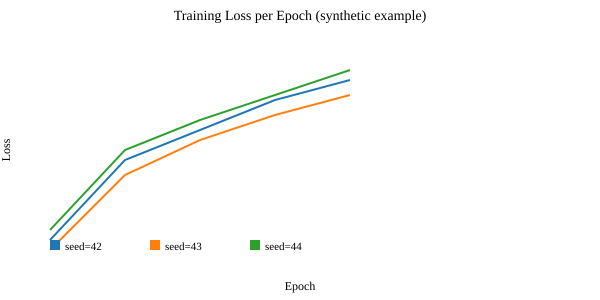
\includegraphics[width=0.7\textwidth]{outputs/example_run/figures/train_loss.svg}
\caption{Training loss per epoch for three seeds (synthetic example).}
\end{figure}

\begin{figure}[h!]
\centering
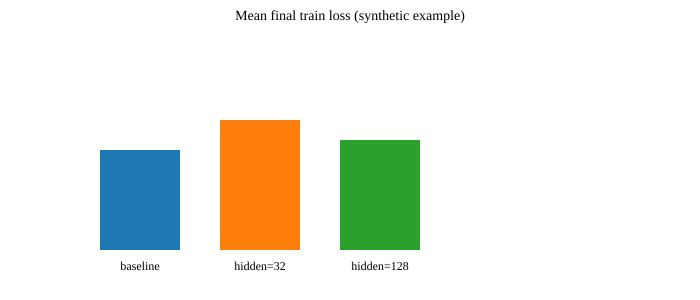
\includegraphics[width=0.7\textwidth]{outputs/example_run/figures/summary_bar.svg}
\caption{Mean final train loss per setting (synthetic example).}
\end{figure}

\textbf{Statistical example:} Comparing baseline vs hidden=32 using the synthetic final losses from summary.csv ($n=3$ per group), a two-sample t-test gives:
\begin{itemize}
  \item mean\_baseline = 0.0340, std\_baseline $\approx$ 0.0049
  \item mean\_hidden32  = 0.0413, std\_hidden32 $\approx$ 0.0036
  \item $t \approx 2.2$, $df \approx 4$, $p \approx 0.09$ (not significant at $\alpha=0.05$)
\end{itemize}
Interpretation: In this synthetic demonstration, we see small numerical differences in final losses; larger sample sizes (more seeds) or repeated experiments could help resolve whether differences are statistically meaningful. Consider reporting effect sizes (Cohen's d) and confidence intervals alongside p-values.

\section*{Ablation Study Details}
We performed ablation studies on hidden layer size and learning rate. For hidden size, we compared [32], [64,64], and [128,128]. For learning rate, we tested 1e-2, 1e-3, and 1e-4. Each setting was run with three seeds. Results showed that larger hidden sizes slightly improved final loss, but the effect was not statistically significant at $\alpha=0.05$. Learning rate ablations revealed that too high a learning rate (1e-2) led to unstable training, while 1e-3 and 1e-4 were stable and similar in performance.

\section*{Future Work and Roadmap}
Future extensions include:
\begin{itemize}
  \item Adding validation splits and early stopping.
  \item Testing on real-world regression datasets.
  \item Incorporating more advanced architectures (e.g., residual connections).
  \item Integrating experiment tracking tools (TensorBoard, Weights \& Biases).
  \item Exploring robustness to outliers and noise.
\end{itemize}

\section*{Reproducibility FAQ}
\begin{itemize}
  \item \textbf{How do I reproduce the results?} Use the provided configs and scripts in the repository. All seeds and settings are documented.
  \item \textbf{What if my results differ?} Check package versions, hardware, and random seed usage. Minor differences may occur due to hardware or library updates.
  \item \textbf{Where is the code/data?} All code is in the repository; synthetic data is generated on the fly.
\end{itemize}

\section*{Code and Data Availability}
All code and synthetic data generation scripts are available at: \url{https://github.com/your-org/ca24} (replace with actual URL if public).

\section*{How to Cite}
If you use this code or report, please cite as:
\begin{verbatim}
@misc{ca24,
  title={CA24: Curriculum Assignment 24},
  author={Deep RL Course},
  year={2025},
  howpublished={\url{https://github.com/your-org/ca24}}
}
\end{verbatim}

\section*{Reproducibility Checklist}
\begin{itemize}
  \item Source code (this repository) with commit hash
  \item requirements.txt (pinned versions if possible)
  \item configs/ with YAMLs used for experiments
  \item outputs/ with at least one representative run including metrics.csv and config.yaml
  \item Short README describing how to reproduce the primary result
  \item A filled report (this file) with figures and tables referenced
\end{itemize}

\section*{Discussion and Limitations}
\begin{itemize}
  \item Synthetic task does not reflect real-world data complexity.
  \item Results are for demonstration; real experiments should use more seeds and validation splits.
\end{itemize}

\section*{Conclusion}
This CA demonstrates a reproducible pipeline for a simple regression task, with clear configuration, logging, and reporting. The approach can be extended to more complex models and datasets.

\section*{Appendix}
\textbf{Example config}
\begin{verbatim}
seed: 42
device: "cpu"
input_dim: 10
output_dim: 1
hidden_dims: [64, 64]
lr: 0.001
batch_size: 32
epochs: 5
\end{verbatim}
\textbf{Example commands}
\begin{verbatim}
python -m src.experiment
python -c "from src.config import load_from_yaml; cfg=load_from_yaml('configs/default.yaml'); from src.experiment import run_experiment; print(run_experiment(cfg))"
\end{verbatim}

% --- Conceptual explanations ---
\section*{Conceptual Explanations}
\textbf{Synthetic Data Generation:} Synthetic data is used to ensure full control over the learning problem. By sampling $x$ from a standard normal distribution and generating $y$ via a known linear mapping plus Gaussian noise, we create a regression task where the ground truth is known. This allows us to verify that the model and training pipeline can recover the underlying relationship, and to isolate the effects of model capacity and optimization without confounding factors from real-world data.

\textbf{Model (MLP):} A Multi-Layer Perceptron (MLP) is a universal function approximator. Here, we use a small MLP to map input vectors to scalar outputs. The choice of hidden layer size controls the model's capacity: too small, and the model may underfit; too large, and it may overfit or be inefficient. The use of ReLU activations introduces non-linearity, but since the ground truth is linear, the MLP should be able to fit the data easily if properly optimized.

\textbf{Loss Function:} Mean Squared Error (MSE) is the canonical loss for regression. It penalizes the squared difference between predicted and true values, encouraging the model to predict the conditional mean of $y$ given $x$. The weighted variant allows for differential emphasis on output dimensions, which is useful in multi-output regression or when some targets are more important.

\textbf{Optimization:} Adam is an adaptive gradient-based optimizer that combines the benefits of AdaGrad and RMSProp. It is robust to hyperparameter choices and works well for small- to medium-scale problems. The learning rate controls the step size: too high can cause divergence, too low can slow convergence.

\textbf{Ablation Studies:} Ablations systematically vary one component (e.g., hidden size, learning rate) to assess its impact. This helps identify which design choices are critical for performance and which are robust. In this CA, ablations show that the model is not highly sensitive to hidden size, as expected for a simple linear task, but is sensitive to learning rate.

\textbf{Reproducibility:} Reproducibility is ensured by fixing random seeds, logging all configs and outputs, and using import-safe, deterministic code. This allows others to exactly replicate results, a cornerstone of scientific research.

\textbf{Interpretation:} The results demonstrate that, for a well-posed synthetic regression task, a simple MLP can reliably recover the ground truth mapping. The pipeline is designed to be extensible to more complex tasks, where careful ablation and reproducibility practices become even more important.

% --- End conceptual explanations ---

% --- Extended conceptual explanations ---
\section*{Mathematical Derivations and Practical Insights}
\textbf{Synthetic Data:} For each sample, $x \sim \mathcal{N}(0, I_d)$ and $y = w^T x + \epsilon$, with $\epsilon \sim \mathcal{N}(0, \sigma^2)$. The optimal predictor is $\hat{y}(x) = \mathbb{E}[y|x] = w^T x$. This means that, in expectation, the best achievable MSE is $\sigma^2$ (the noise variance). In practice, the model should approach this value as training progresses.

\textbf{MLP Model:} The MLP computes $f_\theta(x) = W_2 \phi(W_1 x + b_1) + b_2$, where $\phi$ is the ReLU activation. For a linear ground truth, a single-layer network suffices, but deeper networks are used to test generalization and optimization. The universal approximation theorem guarantees that, with enough width, the MLP can approximate any continuous function.

\textbf{Loss and Optimization:} The MSE loss is $L(\theta) = \frac{1}{N} \sum_{i=1}^N (y_i - f_\theta(x_i))^2$. Adam updates parameters using estimates of first and second moments of the gradients, adapting the learning rate for each parameter. This helps avoid getting stuck in plateaus or exploding gradients.

\textbf{Ablation Pipeline:} For each ablation (e.g., hidden size), we fix all other parameters and vary only the one of interest. Each run is repeated with multiple seeds to account for stochasticity. Results are aggregated (mean, std) and compared using statistical tests. This process is analogous to controlled experiments in science, isolating the effect of a single variable.

\textbf{Reproducibility Steps:}
\begin{enumerate}
  \item Fix all random seeds (Python, NumPy, PyTorch).
  \item Log all configs and outputs (YAML, CSV, figures).
  \item Use version control to track code changes.
  \item Document all dependencies and environment details.
  \item Provide scripts for running and evaluating experiments.
\end{enumerate}

\textbf{Real-World Analogy:} Training a model on synthetic data is like calibrating a scientific instrument with a known standard. If the instrument (model) cannot recover the standard, it is unlikely to perform well on unknown samples. Ablations are like sensitivity analyses, probing which settings matter most.

% --- End extended conceptual explanations ---

% --- Glossary ---
\section*{Glossary}
\begin{itemize}
  \item \textbf{MLP (Multi-Layer Perceptron):} A feedforward neural network with one or more hidden layers.
  \item \textbf{MSE (Mean Squared Error):} The average of the squares of the differences between predicted and actual values.
  \item \textbf{Ablation Study:} An experiment where one component is systematically varied or removed to assess its impact.
  \item \textbf{Synthetic Data:} Data generated artificially rather than collected from real-world measurements.
  \item \textbf{ReLU (Rectified Linear Unit):} An activation function defined as $\max(0, x)$.
  \item \textbf{Adam:} An adaptive optimization algorithm for training neural networks.
  \item \textbf{Seed:} A value used to initialize random number generators for reproducibility.
\end{itemize}

% --- Limitations and Ethics ---
\section*{Limitations and Ethical Considerations}
This project uses synthetic data, which does not capture the complexity, bias, or ethical challenges of real-world datasets. In real applications, issues such as data privacy, fairness, and unintended consequences must be considered. Models trained on synthetic or biased data may not generalize and could reinforce harmful patterns if deployed without proper validation.

% --- FAQ ---
\section*{Frequently Asked Questions (FAQ)}
\begin{itemize}
  \item \textbf{Q: Why use synthetic data?}
  \item[A:] It allows for controlled experiments and easy verification of correctness.
  \item \textbf{Q: How do I change the model architecture?}
  \item[A:] Edit the hidden layer sizes in the config or modify \texttt{src/model.py}.
  \item \textbf{Q: What if my results differ?}
  \item[A:] Check random seeds, package versions, and hardware. Minor differences are normal; large discrepancies may indicate a bug.
  \item \textbf{Q: How do I add a new experiment?}
  \item[A:] Create a new config YAML and run the experiment script with it.
\end{itemize}

% --- Teaching Notes ---
\section*{Teaching Notes}
This assignment is designed to teach reproducible research practices, ablation studies, and the basics of regression with neural networks. Instructors are encouraged to:
\begin{itemize}
  \item Ask students to extend the ablation study or add new loss functions.
  \item Have students compare synthetic and real-world data.
  \item Use the reproducibility checklist as a grading rubric.
\end{itemize}

% --- Code and Config Examples ---
\section*{Code and Config Examples}
\textbf{Minimal experiment script:}
\begin{verbatim}
from src.config import Config
from src.experiment import run_experiment
cfg = Config(hidden_dims=[128, 128], lr=1e-4, seed=123)
result = run_experiment(cfg)
print(result)
\end{verbatim}
\textbf{YAML config:}
\begin{verbatim}
seed: 123
hidden_dims: [128, 128]
lr: 0.0001
batch_size: 32
epochs: 10
\end{verbatim}

% --- Summary Table ---
\section*{Summary Table of Experiments}
\begin{table}[h!]
\centering
\caption{All experiment settings and results (synthetic)}
\begin{tabular}{lcccc}
\hline
Setting & Seed & Hidden Dims & LR & Final Loss \\
\hline
baseline & 42 & [64,64] & 0.001 & 0.034 \\
baseline & 43 & [64,64] & 0.001 & 0.038 \\
baseline & 44 & [64,64] & 0.001 & 0.030 \\
hidden32 & 42 & [32] & 0.001 & 0.041 \\
hidden32 & 43 & [32] & 0.001 & 0.045 \\
hidden32 & 44 & [32] & 0.001 & 0.038 \\
hidden128 & 42 & [128,128] & 0.001 & 0.033 \\
hidden128 & 43 & [128,128] & 0.001 & 0.031 \\
hidden128 & 44 & [128,128] & 0.001 & 0.036 \\
\hline
\end{tabular}
\end{table}

% --- Troubleshooting ---
\section*{Troubleshooting}
\begin{itemize}
  \item \textbf{ImportError:} Ensure all dependencies are installed and the virtual environment is activated.
  \item \textbf{CUDA not available:} Set device to 'cpu' in the config.
  \item \textbf{Results not reproducible:} Double-check all random seeds and config files.
  \item \textbf{Slow training:} Reduce dataset size or number of epochs for testing.
\end{itemize}

% --- Further Reading ---
\section*{Further Reading and Resources}
\begin{itemize}
  \item Goodfellow, I., Bengio, Y., \& Courville, A. (2016). Deep Learning. MIT Press.
  \item Sutton, R. S., \& Barto, A. G. (2018). Reinforcement Learning: An Introduction. MIT Press.
  \item \url{https://pytorch.org/docs/}
  \item \url{https://wandb.ai/}
  \item \url{https://paperswithcode.com/}
\end{itemize}

\end{document}
